\documentclass[border=10pt]{standalone}
\usepackage{tikz}
\begin{document}
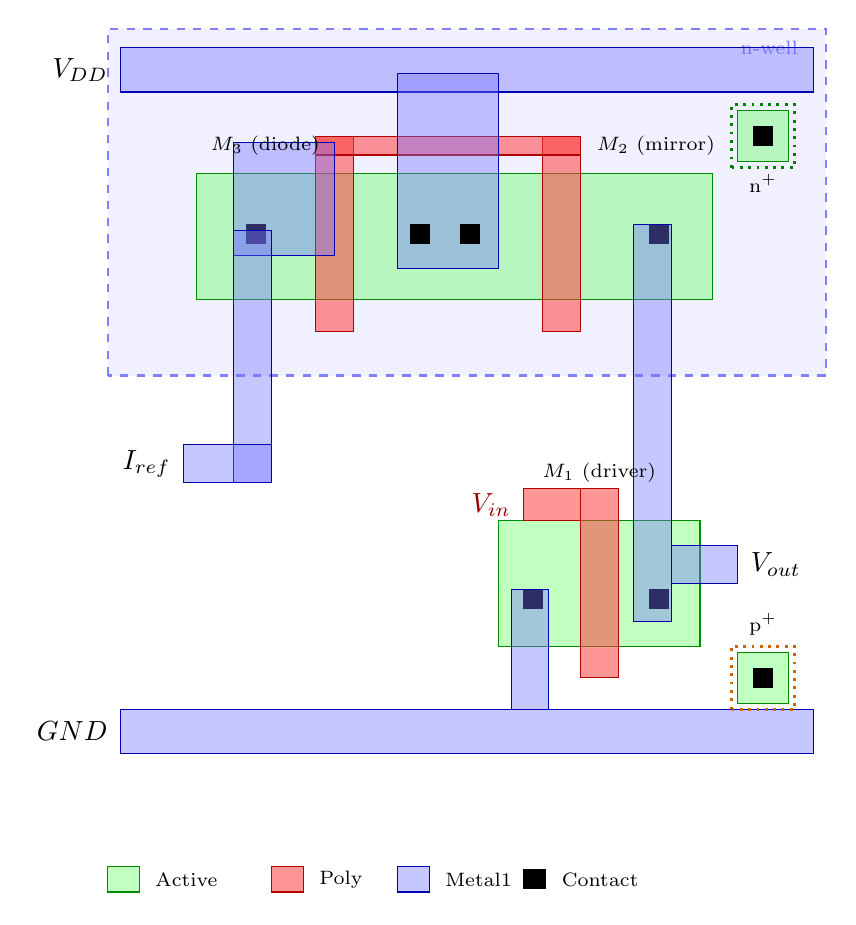
\begin{tikzpicture}[scale=0.8,
  nwell/.style ={draw=blue!50, dashed, line width=1pt, fill=blue!6},
  active/.style={draw=green!55!black, fill=green!55, fill opacity=0.45},
  poly/.style  ={draw=red!70!black,  fill=red!75,   fill opacity=0.55},
  metal/.style ={draw=blue!70!black, fill=blue!55,  fill opacity=0.40},
  cont/.style  ={draw=black, fill=black},
  sel/.style   ={draw=#1, dotted, line width=1pt}]

  % n-well (top) holding the PMOS current mirror M2, M3
  \fill[nwell] (0.0,6.3) rectangle (11.4,11.8);
  \node[blue!55] at (10.5,11.5){\scriptsize n-well};

  % rails
  \fill[metal] (0.2,10.8) rectangle (11.2,11.5); \node[left] at (0.15,11.15){$V_{DD}$};
  \fill[metal] (0.2,0.3)  rectangle (11.2,1.0);   \node[left] at (0.15,0.65){$GND$};

  % shared p-diffusion of the mirror : [D_M3 | gM3 | S(VDD) | gM2 | D_M2]
  \fill[active] (1.4,7.5) rectangle (9.6,9.5);
  % two mirror gates (poly), bridged across the top -> common gate
  \fill[poly] (3.3,7.0) rectangle (3.9,10.1);
  \fill[poly] (6.9,7.0) rectangle (7.5,10.1);
  \fill[poly] (3.3,9.8) rectangle (7.5,10.1);          % poly bridge (gates tied)

  % shared source (middle) -> VDD
  \fill[metal] (4.6,8.0) rectangle (6.2,11.1);
  \foreach \x in {4.8,5.6}{\fill[cont] (\x,8.4) rectangle (\x+0.3,8.7);}

  % M3 drain (left) : diode-connect to the gate bridge + reference node
  \fill[cont] (2.2,8.4) rectangle (2.5,8.7);
  \fill[metal] (2.0,8.2) rectangle (3.6,10.0);          % up to poly bridge -> diode
  \fill[metal] (2.0,4.6) rectangle (2.6,8.6);           % down to Iref pad
  \fill[metal] (1.2,4.6) rectangle (2.6,5.2); \node[left] at (1.15,4.9){$I_{ref}$};

  % M2 drain (right) = Vout
  \fill[cont] (8.6,8.4) rectangle (8.9,8.7);

  % ---- NMOS driver M1 (below) : [S=GND | gate | D=Vout] ----
  \fill[active] (6.2,2.0) rectangle (9.4,4.0);
  \fill[poly]   (7.5,1.5) rectangle (8.1,4.5);
  \fill[poly]   (7.5,4.0) rectangle (6.6,4.5); \node[red!60!black,left] at (6.55,4.25){$V_{in}$};
  % M1 drain = Vout (right region) tied to M2 drain via a narrow metal column
  \fill[cont] (8.6,2.6) rectangle (8.9,2.9);
  \fill[metal] (8.35,2.4) rectangle (8.95,8.7);         % Vout column: M2 drain -> M1 drain
  \fill[metal] (8.95,3.0) rectangle (10.0,3.6); \node[right] at (10.05,3.3){$V_{out}$};
  % M1 source -> GND (left region)
  \fill[cont] (6.6,2.6) rectangle (6.9,2.9);
  \fill[metal] (6.4,1.0) rectangle (7.0,2.9);

  % well tap (n+)->VDD  &  substrate tap (p+)->GND
  \fill[active] (10.0,9.7) rectangle (10.8,10.5); \draw[sel=green!50!black](9.9,9.6)rectangle(10.9,10.6);
  \fill[cont] (10.25,9.95) rectangle (10.55,10.25); \node at (10.4,9.35){\scriptsize n$^{+}$};
  \fill[active] (10.0,1.1) rectangle (10.8,1.9); \draw[sel=orange!80!black](9.9,1.0)rectangle(10.9,2.0);
  \fill[cont] (10.25,1.35) rectangle (10.55,1.65); \node at (10.4,2.35){\scriptsize p$^{+}$};

  % device labels
  \node at (2.5,9.95){\scriptsize $M_3$ (diode)};
  \node at (8.7,9.95){\scriptsize $M_2$ (mirror)};
  \node at (7.8,4.75){\scriptsize $M_1$ (driver)};

  % legend
  \begin{scope}[shift={(0,-2.4)}]
    \fill[active](0,0.5) rectangle(0.5,0.9); \node[right] at(0.6,0.7){\scriptsize Active};
    \fill[poly]  (2.6,0.5) rectangle(3.1,0.9); \node[right] at(3.2,0.7){\scriptsize Poly};
    \fill[metal] (4.6,0.5) rectangle(5.1,0.9); \node[right] at(5.2,0.7){\scriptsize Metal1};
    \fill[cont]  (6.6,0.55) rectangle(6.95,0.85); \node[right] at(7.05,0.7){\scriptsize Contact};
  \end{scope}
\end{tikzpicture}
\end{document}
